\documentclass{article}
\usepackage{crysymb}
\usepackage{graphics}
\usepackage{amsthm}
\usepackage[pdftex]{graphicx} 

\newtheorem{claim}{Claim}
\newtheorem{theorem}{Theorem}


\renewcommand{\vec}[1]{\boldsymbol{#1}}
\newcommand{\pd}[1]{\mathrm{p}[#1]}
\newcommand{\supi}[1]{^{\scriptscriptstyle(#1)}}

\DeclareMathOperator*{\argmax}{argmax}
\DeclareMathOperator*{\argmin}{argmin}

\title{\textsc{Expectation-Maximisation Algorithm}\\ Derivation and a cookbook for further recepies}
\author{Sven Laur\\ University of Tartu \\ email \texttt{swen@math.ut.ee}}

\begin{document}
\maketitle
\section{Mixture model}

To simplify the treatment, we consider here only how to derive and apply the expectation-maximisation algorithm in the context of soft clustering. The treatment of other applications is analogous. The soft-clustering is based on a probabilistic model, which combines $k$ different data sources. More precisely, we assume that individual observations $\vec{x}_1,\ldots,\vec{x}_n$ are generated by $k$ different data sources $\DDD_1,\ldots,\DDD_k$. Each data source $\DDD_j$ is modelled by a probability distribution with parameters $\vec{\Theta}_j$ and thus we can always compute the likelihood $\pd{\vec{x}_i|\vec{\Theta}_j}$. Furthermore, we assume that all data points are independently sampled and the probability that $\vec{x}_i$ is generated by the data source $\DDD_j$ is $\lambda_j$. These parameters are also known as mixture proportions. Now let
\begin{align*}
\vec{\Theta}=(\lambda_1,\ldots,\lambda_k,\vec{\Theta}_1,\ldots,\vec{\Theta}_k)
\end{align*}
denote the set of all parameters. Then it is straightforward to estimate the likelihood of an individual observation
\begin{align*}
\pd{\vec{x}_i|\vec{\Theta}}=\sum_{j=1}^k\lambda_j\cdot\pd{\vec{x}_i|\vec{\Theta}_j}\enspace.
\end{align*}
As a concrete example, consider a two-dimensional mixture model where both components are a two-dimensional normal distributions  with parameters:   
\begin{align*}
\Sigma_1&=
\begin{pmatrix}
 \phantom{-}4.125   &-3.875\\
 -3.875 &\phantom{-}4.125
\end{pmatrix}\enspace
\qquad
\vec{\mu}_1=
\begin{pmatrix}
\phantom{-}4\\
-4
\end{pmatrix}\enspace\\
\Sigma_2&=
\begin{pmatrix}
 \phantom{-}4.125   &\phantom{-}3.875\\
 \phantom{-}3.875 &\phantom{-}4.125
\end{pmatrix}\enspace
\qquad
\vec{\mu}_2=
\begin{pmatrix}
-4\\
\phantom{-}4
\end{pmatrix}\enspace
\end{align*}
and equal mixture proportions:
\begin{align*}
\lambda_1&=0.5 &
\lambda_2&=0.5\enspace.
\end{align*} 
The corresponding model is depicted in Figure~\ref{fig:gmm}.



\begin{figure}[!t]
\begin{center}
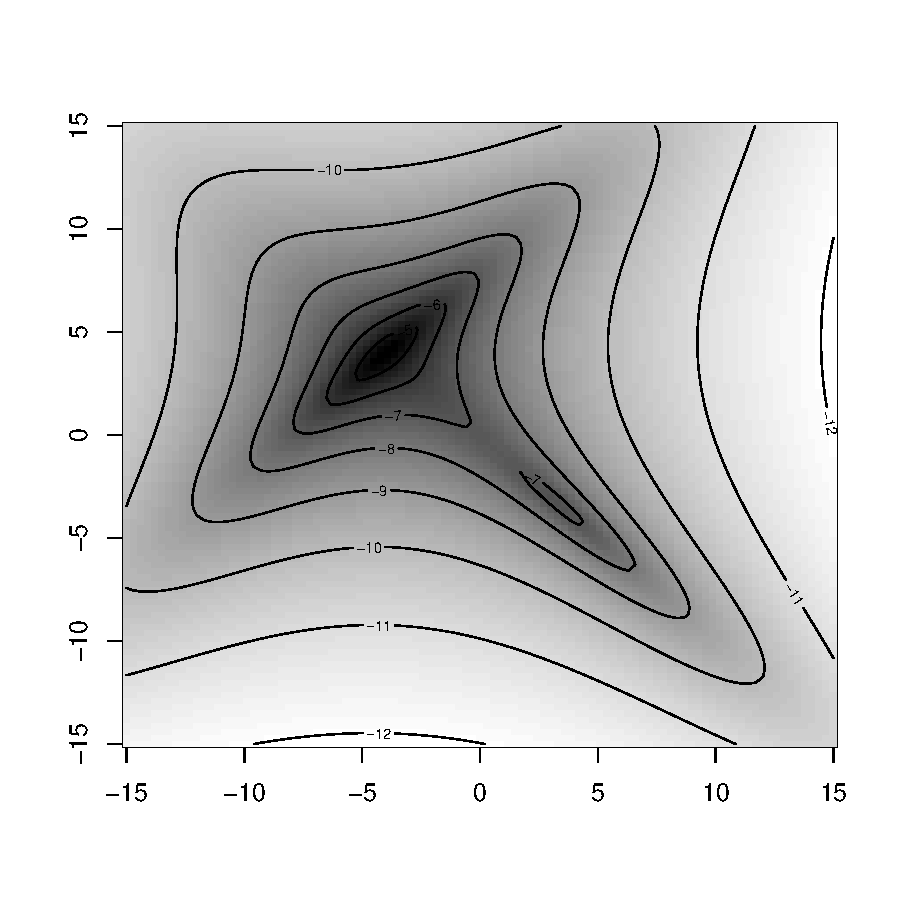
\includegraphics[width=6cm,trim=1cm 1.5cm 0cm 1.0cm, clip]{illustrations/gmm-example-i.pdf}\hspace*{0cm}
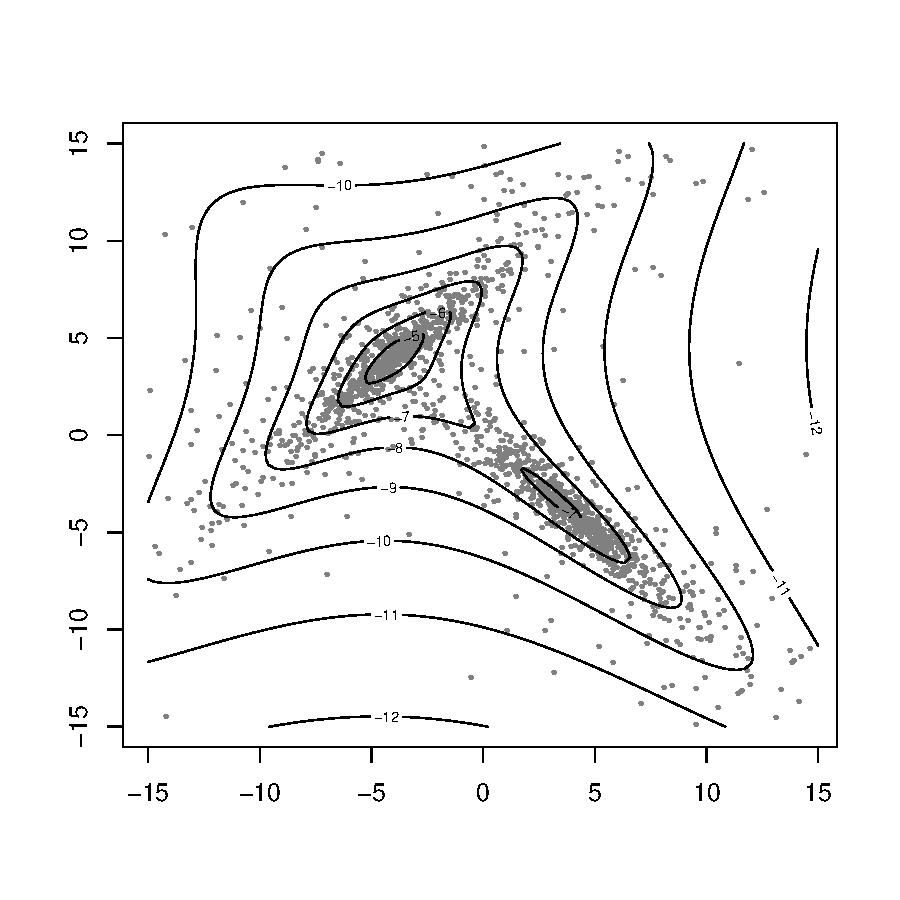
\includegraphics[width=6cm,trim=1cm 1.5cm 0cm 1.0cm, clip]{illustrations/gmm-example-ii.pdf}
\end{center}
\caption{Two-dimesnional Gaussian mixture model. Probability density function is depicted on the left and $2000$ element sample is depicted on the right.}
\label{fig:gmm}
\end{figure}

\section{Approximation of log-likelihood}

Let $\vec{z}=(z_1,\ldots,z_n)$ denote a potential labelling of points where $z_i\in\set{1,\ldots,k}$ shows from which data source $\DDD_j$ the datapoint $\vec{x}_i$ is generated. For brevity, let 
\begin{align*}
\ZZZ=\set{1,\ldots,k}^n
\end{align*} 
denote the set of all possible labelings. Then the posterior distribution of model parameters     
\begin{align}\label{eq:posterior}
\pd{\vec{\Theta}|\vec{x}_1,\ldots\vec{x}_n}&=\sum_{\vec{z}\in\ZZZ}\pd{\vec{\vec{z},\Theta}|\vec{x}_1,\ldots,\vec{x}_n}
\end{align}
can be further decomposed by applying product rule to individual terms 
\begin{align*}
\pd{\vec{\vec{z},\Theta}|\vec{x}_1,\ldots,\vec{x}_n} = %
\pr{\vec{\vec{z}|\Theta},\vec{x}_1,\ldots,\vec{x}_n}\cdot
\pd{\vec{\Theta}|\vec{x}_1,\ldots,\vec{x}_n}  
\end{align*}
where the first term assigns probabilities to individual labelings and the second term is the term we want to express\footnote{Although it is formally correct we have gotten nowhere, yet}. Let us assume that we have somehow gotten a rather good estimate $q: \ZZZ\to \RR$ on the labelling probabilities, i.e.,
\begin{align*}
\forall z\in\ZZZ:\qquad q(\vec{z})\approx \pr{\vec{\vec{z}|\Theta},\vec{x}_1,\ldots,\vec{x}_n}\enspace 
\end{align*} 
and we want to use and improve this estimation further. Without loss of generality, we can assume that the approximation is a proper probability distribution: 
\begin{align}\label{eq:z-normalisation}
 \sum_{\vec{z}\in\ZZZ}q(\vec{z})=1\enspace.
\end{align}
If $q(\vec{z})$ is not a probability distribution, we can always renormalise it. The latter does not change the values much, since   
\begin{align*}
 \sum_{\vec{z}\in\ZZZ}\pr{\vec{z}|\vec{\Theta},\vec{x_1},\ldots,\vec{x}_n}=1\enspace.
\end{align*}

Under this assumptions, we can approximate the sought posterior probability using individual labellings $\vec{z}$: 
\begin{align}\label{eq:approx-assumption}
\pd{\vec{\Theta}|\vec{x}_1,\ldots,\vec{x}_n}=%
\frac{\pd{\vec{\vec{z},\Theta}|\vec{x}_1,\ldots,\vec{x}_n}}{\pd{\vec{\vec{z}|\Theta},\vec{x}_1,\ldots,\vec{x}_n}} \approx %
\frac{\pd{\vec{\vec{z},\Theta}|\vec{x}_1,\ldots,\vec{x}_n}}{q(\vec{z})}
\end{align}
By substituting both approximations into the equation~\eqref{eq:posterior}, we get another circular statement which is obvious:
\begin{align*}
\pd{\vec{\Theta}|\vec{x}_1,\ldots\vec{x}_n}&=\sum_{\vec{z}\in\ZZZ} q(\vec{z})\cdot
\frac{\pd{\vec{\vec{z},\Theta}|\vec{x}_1,\ldots,\vec{x}_n}}{q(\vec{z})}\enspace.
\end{align*}
To maximise this, we can take logarithms form both sides and maximise the right hand side of the following statement  
\begin{align*}
\log\pd{\vec{\Theta}|\vec{x}_1,\ldots\vec{x}_n}&=\log\left(\sum_{\vec{z}\in\ZZZ} q(\vec{z})\cdot
\frac{\pd{\vec{\vec{z},\Theta}|\vec{x}_1,\ldots,\vec{x}_n}}{q(\vec{z})}\right)\enspace.
\end{align*}
Since logarithm is a convex-cap function, the Jensen inequality allows us to push the logarithm through the sum to get a lower bound
\begin{align}\label{eq:lower-bound}
F(q,\vec{\Theta}):=\sum_{\vec{z}\in\ZZZ} q(\vec{z})\cdot
\log\left(\frac{\pd{\vec{\vec{z},\Theta}|\vec{x}_1,\ldots,\vec{x}_n}}{q(\vec{z})}\right)\leq
\log\pd{\vec{\Theta}|\vec{x}_1,\ldots\vec{x}_n}
\enspace.
\end{align}


As $q(\vec{z})$ is a good approximation of $\pd{\vec{z}|\vec{\Theta},\vec{x}_1,\ldots,\vec{x}_n}$,
we can use the approximation~\eqref{eq:approx-assumption} to 
show that the lower bound $F(q,\vec{\Theta})$ is close to to the actual value. Indeed, note that
\begin{align*}
\sum_{\vec{z}\in\ZZZ} q(\vec{z})\cdot
\log\left(\frac{\pd{\vec{\vec{z},\Theta}|\vec{x}_1,\ldots,\vec{x}_n}}{q(\vec{z})}\right)
&\approx \sum_{\vec{z}\in\ZZZ} q(\vec{z})\cdot \log\bigl(\pd{\vec{\Theta}|\vec{x}_1,\ldots,\vec{x}_n}\bigr)
\end{align*}
which together with the equation~\eqref{eq:z-normalisation} itself implies
\begin{align*}
\sum_{\vec{z}\in\ZZZ} q(\vec{z})\cdot
\log\left(\frac{\pd{\vec{\vec{z},\Theta}|\vec{x}_1,\ldots,\vec{x}_n}}{q(\vec{z})}\right)&\approx \log\bigl(\pd{\vec{\Theta}|\vec{x}_1,\ldots,\vec{x}_n}\bigr)
\end{align*}
To summarise, we have shown the following important claim.

\begin{claim}
Assume that $q(\vec{z})$ is a good approximation of a posterior probability $\pr{\vec{z}|\vec{\Theta},\vec{x}_1,\ldots,\vec{x}_n}$. Then the lower bound $F(q,\vec{\Theta})\approx\log\bigl(\pd{\vec{\Theta}|\vec{x}_1,\ldots,\vec{x}_n}\bigr)$. 
\end{claim} 

\section{Iterative minimisation algorithm}

In most cases, exact minimisation of the log-likelihood $\pd{\vec{\Theta}|\vec{x}_1,\ldots,\vec{x}_n}$ is intractable and even the exact computation of partial derivatives for the iterative minimisation is a challenging task. Hence, the iterative minimisation of $F(q,\vec{\Theta})$ together with the recalibration of the approximation $q(\vec{z})$ on the posterior probability $\pr{\vec{z}|\vec{\Theta},\vec{x}_1,\ldots,\vec{x}_n}$ is a compelling alternative, see Figure~\ref{fig:iterative-approximation}.

\begin{figure}[!t]
\begin{center}
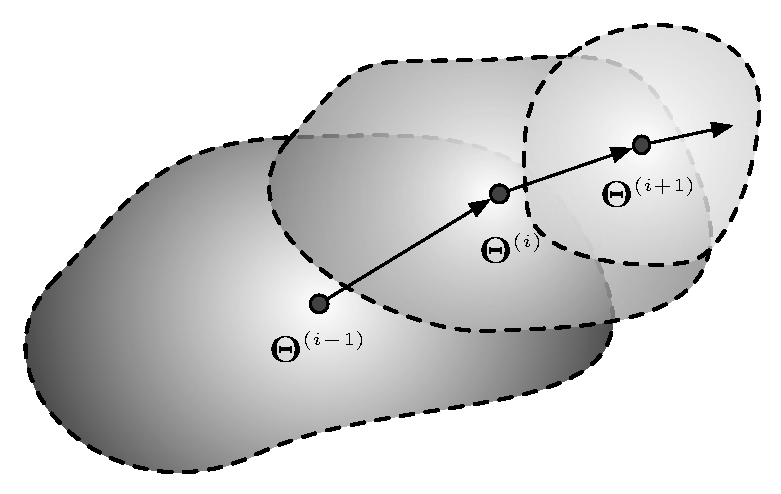
\includegraphics[width=8cm]{illustrations/em-approximation}
\end{center}
\caption{Iterative approximate search for maximal a posteriori estimate. Given a current solution $\vec{\Theta}\supi{i}$, approximate the log-likelihood and find the next optimum $\vec{\Theta}^{(i+1)}$. The algorithm is guaranteed to work if the new solution $\vec{\Theta}\supi{i+1}$ is inside the grey region where the approximation is good. In each step, we have to recalibrate the approximation by setting $q(\vec{z})=\pr{\smash{\vec{z}|\vec{\Theta}\supi{i},\vec{x}_1,\ldots,\vec{x}_n}}$.   }
\label{fig:iterative-approximation}
\end{figure}      

Let us study this iterative maximisation procedure in more detail. In particular, let $q_{i}(\vec{z})=\pr{\smash{\vec{z}|\vec{\Theta}\supi{i},\vec{x}_1,\ldots,\vec{x}_n}}$ and $q_{i+1}(\vec{z})=\pr{\smash{\vec{z}|\vec{\Theta}\supi{i+1},\vec{x}_1,\ldots,\vec{x}_n}}$ be the approximations of the labelling distributions used in steps $i$ and $i+1$. 
Then the next value of parameters is computed by maximising the lower bound:
\begin{align}\label{eq:choice-of-theta}
\vec{\Theta}\supi{i+1}=\argmax_{\vec{\Theta}} F(q_{i},\vec{\Theta})\enspace.
\end{align}
Let us assume further that  $\vec{\Theta}\supi{i+1}$ is so close to $\vec{\Theta}\supi{i}$ that
\begin{align*}
q_{i}(\vec{z})\approx q_{i+1}(\vec{z})\enspace.
\end{align*}
Then Claim~1 assures that the lower bound is rather close to the actual log-likelihood:
\begin{align*}
F(q_{i},\vec{\Theta}\supi{i+1})\approx\log\bigl(\pd{\vec{\Theta}\supi{i+1}|\vec{x}_1,\ldots,\vec{x}_n}\bigr)\enspace.
\end{align*} 
Moreover, the approximation becomes more and more accurate if the difference between individual steps converges to zero: 
\begin{align*}
\norm{\vec{\Theta}\supi{i}-\vec{\Theta}\supi{i+1}}\to 0\enspace.
\end{align*} 

\begin{figure}[!ht]
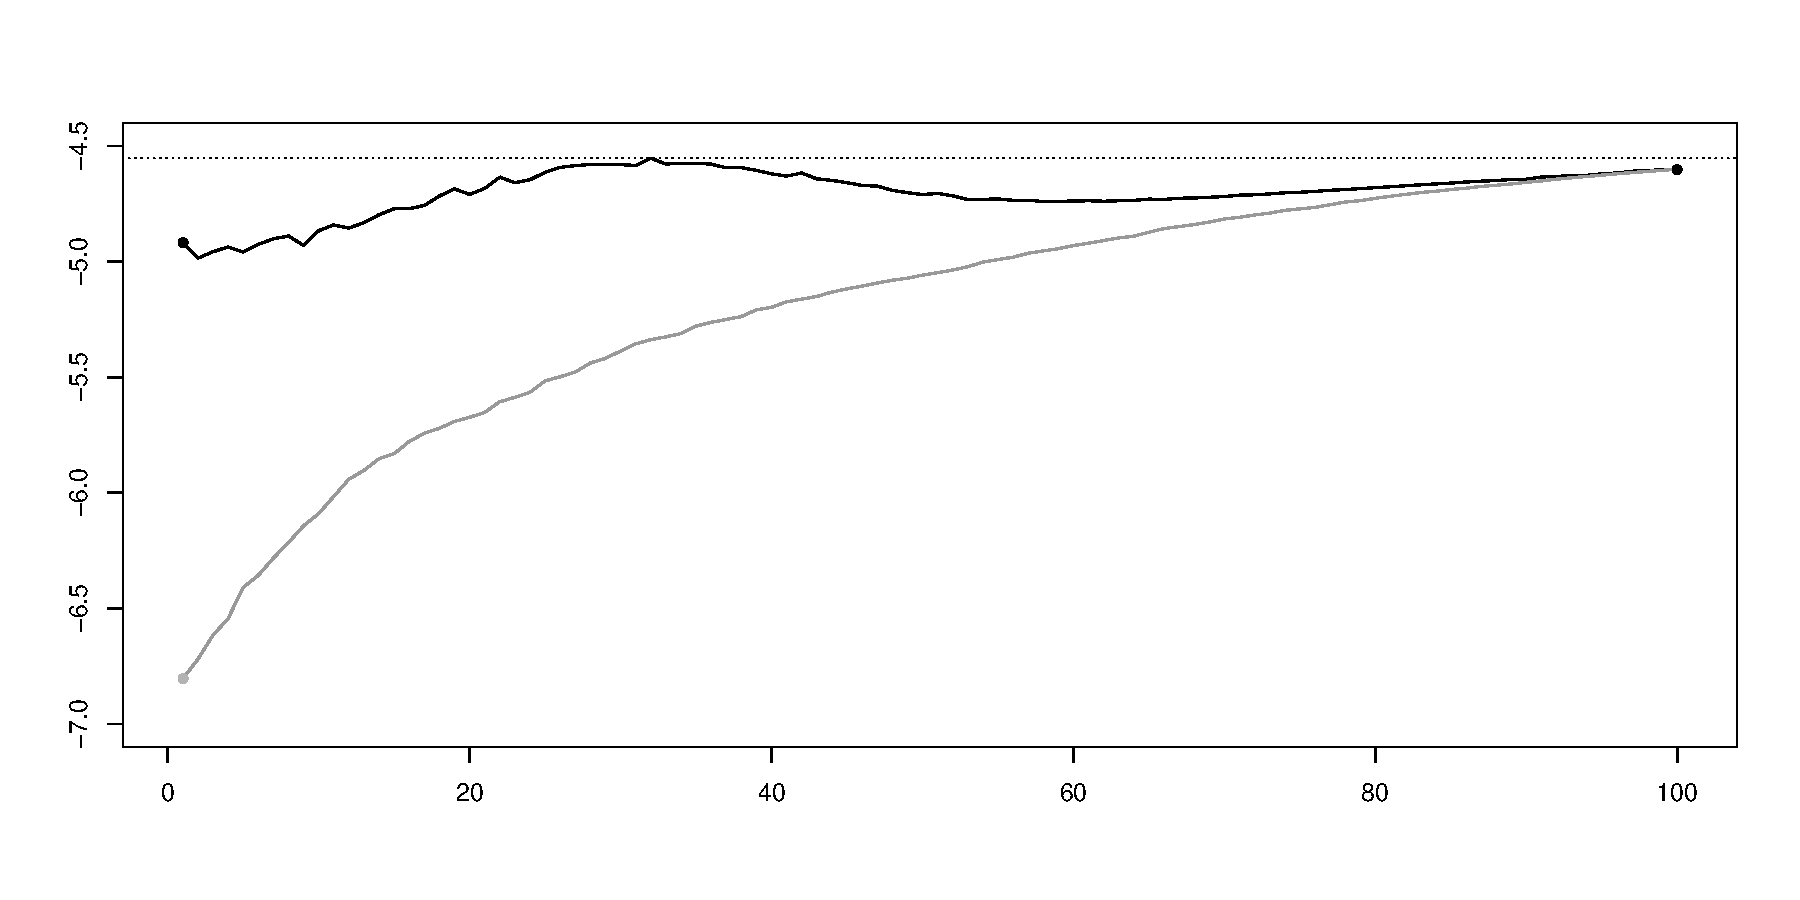
\includegraphics[width=12cm]{illustrations/em-convergence}
\caption{Convergence of the EM-algorithm. The $x$-axis depicts iterations. The $y$-axis depicts the values of the log-likelihood and its lower bound. The grey line shows how the lower bound increases during iterative minimisation. The black line shows the maximal value of the log-likelihood in a fixed size surrounding of $\vec{\Theta}\supi{i}$. The iterative maximisation quickly converges to a local maxima. However, it also misses a another maximum, since this maximum is rather far away from the search path and thus the approximation is not good enough to detect it.  }
\label{fig:em-bound-convergence}
\end{figure}


As a direct consequence note that if we manage to show that the iterative maximisation procedure converges
\begin{align*}
\vec{\Theta}\supi{i} \to \vec{\Theta}^*
\end{align*}
then also the lower bound converges to the log-likelihood:
\begin{align*}
F(q_i,\vec{\Theta}\supi{i}) \to \log\bigl(\pd{\vec{\Theta}^*|\vec{x}_1,\ldots,\vec{x}_n}\bigr)
\end{align*}
Moreover, as $\vec{\Theta}^*$ is the local maximum of the lower bound $F(q_*,\vec{\Theta})$ then it must be also a local    
maximum of $\log\bigl(\pd{\vec{\Theta}|\vec{x}_1,\ldots,\vec{x}_n}\bigr)$.  Informal reasoning is the following. In a small surrounding of $\vec{\Theta}^*$, the approximation 
\begin{align*}
F(q_*,\vec{\Theta}) \approx \log\bigl(\pd{\vec{\Theta}|\vec{x}_1,\ldots,\vec{x}_n}\bigr)
\end{align*}
is so good that the maximum condition
\begin{align*}
F(q_*,\vec{\Theta})\leq F(q_*,\vec{\Theta}^*)  
\end{align*}
also implies the same for log-likelihoods
\begin{align*}
\log\bigl(\pd{\vec{\Theta}|\vec{x}_1,\ldots,\vec{x}_n}\bigr) \leq \log\bigl(\pd{\vec{\Theta}^*|\vec{x}_1,\ldots,\vec{x}_n}\bigr)\enspace.
\end{align*}
These basic concepts behind the algorithm are illustrated in Figure~\ref{fig:em-bound-convergence}. 


\section{Expectation-Maximisation algorithm}

\begin{figure}[!t]
\begin{center}
\frame{
\begin{minipage}{12cm}
\vspace*{1ex}
\begin{tabbing}
\hspace*{12cm}\\
\hspace*{1em}\=\=\kill
\>1. Choose a suitable initial estimate for model parameters $\vec{\Theta}\supi{0}$.\\
\>2. \textsc{E-step.} Given an estimate $\vec{\Theta}\supi{t}$ update labelling probability:
\end{tabbing}
\begin{align*}
\forall \vec{z}\in\ZZZ:\qquad q_t(\vec{z})=\pr{\smash{\vec{z}|\vec{\Theta}\supi{t},\vec{x}_1,\ldots,\vec{x}_n}}\enspace.
\end{align*}
\begin{tabbing}
\hspace*{1em}\=\=\kill
\>3. \textsc{M-step.} Find the next estimate $\vec{\Theta}\supi{t+1}$ by minimising the lower bound:
\end{tabbing}\vspace*{-1ex}
\begin{align*}
\vec{\Theta}\supi{t+1}=\argmax_{\vec{\Theta}} F(q_{t},\vec{\Theta})\enspace.
\end{align*}
\begin{tabbing}
\hspace*{1em}\=\=\kill
\>4. Repeat from the step 2 until convergence.\\ 
\end{tabbing}
\vspace*{1ex}
\end{minipage}}
\end{center}
\caption{Expectation-maximisation algorithm}
\label{fig:em-algorithm} 
\end{figure} 


Our treatment of the iterative minimisation algorithm described above was rather informal. In particular, we did not probe that the sequence of iterative updates leads to the sequence of estimates 
\begin{align*}
\vec{\Theta}\supi{0},\vec{\Theta}\supi{1},\ldots,\vec{\Theta}\supi{i},\vec{\Theta}\supi{i+1}\ldots
\end{align*}
that converges to a limiting value $\vec{\Theta}^*$. It is straightforward to see that 
\begin{align*}
F(q_t,\vec{\Theta}\supi{i})\leq F(q_t,\vec{\Theta}\supi{t+1})\enspace.
\end{align*}
since the update step~\eqref{eq:choice-of-theta} maximises $F(q_t, \vec{\Theta})$. However, the recalibration of the labelling probabilities:
\begin{align*}
q_{t+1}(\vec{z})=\pr{\smash{\vec{z}|\vec{\Theta}\supi{t+1},\vec{x}_1,\ldots,\vec{x}_n}}
\end{align*}
is completely detached form $F(q,\vec{\Theta})$ and thus we must do further analysis to show 
\begin{align*}
F(q_t,\vec{\Theta}\supi{t+1})\leq F(q_{t+1},\vec{\Theta}\supi{t+1})\enspace,
\end{align*}
which would assure the convergence since the log-likelihood of the model must be bounded and thus also its lower bound $F(q,\vec{\Theta})$. The corresponding proof can be obtained through straightforward manipulations
\begin{align*}
F(q_{t+1},\vec{\Theta}\supi{t+1})%
&=\sum_{\vec{z}\in\ZZZ} q_{t+1}(\vec{z})\cdot
\log\left(\frac{\pd{\vec{z},\vec{\Theta}\supi{t+1}|\vec{x}_1,\ldots,\vec{x}_n}}
{\pr{\vec{z}|\vec{\Theta}\supi{t+1},\vec{x}_1,\ldots,\vec{x}_n}}\right)\\
&=\sum_{\vec{z}\in\ZZZ} q(\vec{z})\cdot
\log\left(\pd{\vec{\Theta}\supi{t+1}| \vec{x}_1,\ldots,\vec{x}_n}\right)\\ 
&=\log\left(\pd{\vec{\Theta}\supi{t+1}| \vec{x}_1,\ldots,\vec{x}_n}\right)
\end{align*}
where the second equation from the Bayes equation
\begin{align*}
\pd{\vec{\vec{z},\Theta}\supi{t+1}|\vec{x}_1,\ldots,\vec{x}_n} = %
\pr{\vec{\vec{z}|\Theta}\supi{t+1},\vec{x}_1,\ldots,\vec{x}_n}\cdot
\pd{\vec{\Theta}\supi{t+1}|\vec{x}_1,\ldots,\vec{x}_n} \enspace. 
\end{align*}
Hence we have shown that after the recalibration step the lower bound matches the value it bounds:
\begin{align*}
F(q_{i+1},\vec{\Theta}\supi{t+1})=\log(\pr{\vec{\Theta}\supi{i+1}|\vec{x}_1,\ldots,\vec{x}_n})
\end{align*}
and thus also 
\begin{align*}
F(q_{t},\vec{\Theta}\supi{t+1})\leq F(q_{t+1},\vec{\Theta}\supi{t+1})\enspace.
\end{align*}
Hence, we have shown the following claim.

\begin{theorem}
The expectation-maximisation algorithm is guaranteed to converge if the log-likelihood function $\log(\pd{\vec{\Theta}|\vec{x}_1,\ldots,\vec{x}_n})$ is bounded.
\end{theorem} 
\begin{proof}[Proof sketch]
Since both steps of the algorithm increase the lower bound and the log-likelihood is bounded the sequence of values 
\begin{align*}
F(q_{1},\vec{\Theta}\supi{1}),\ldots,
F(q_{i},\vec{\Theta}\supi{i}),\ldots
\end{align*}
must converge to a limiting value. Hence the algorithm will stop. It is much more difficult to formally show that the convergence also takes place in terms of parameters $\vec{\Theta}\supi{0}, \vec{\Theta}\supi{1},\ldots,\vec{\Theta}\supi{i},\ldots$, as large change in arguments might lead to small change in the output. To guarantee convergence in parameters, we must assume regularity from the function, i.e., there are no plateaus of constant values, where the algorithm could get stuck.    
\end{proof}

\section{Semantics behind the maximisation step}

The general description of the M-step is rather void of any meaning. In the following, we show how one can give a fractional semantics to this step. The main difference between the EM-algorithm and the hard clustering algorithm is in the E-step. The hard clustering algorithm chooses the most probable label $z_i$ for the datapoint $\vec{x}_i$ and the proceeds to find optimal parameters for reach cluster. The soft-clustering algorithm assigns weights  
\begin{align*}
w_{ij}=\pr{z_i=j|\vec{x}_i,\vec{\Theta}\supi{t}}\enspace
\end{align*}
to each data point and uses all points with appropriate weighs to re-estimate cluster parameters $\vec{\Theta}$. Next, we will show that the steps in the soft-clustering algorithm correspond to the E-step and the M-step. 

First of all note that the recalibration rule in the E-step can be decomposed further as all data points are assumed to be independently drawn and labelled:  
\begin{align*}
q_{t}(\vec{z})=\frac{\pd{\smash{\vec{z},\vec{x}_1,\ldots,\vec{x}_n|\vec{\Theta}\supi{t}}}}
{\pd{\smash{\vec{x}_1,\ldots,\vec{x}_n|\vec{\Theta}\supi{t}}}}=\prod_{i=1}^n\frac{\pd{\smash{z_i,\vec{x}_i|\vec{\Theta}\supi{t}}}}
{\pd{\smash{\vec{x}_i|\vec{\Theta}\supi{t}}}}=\prod_{i=1}^n \pr{z_i|\vec{x}_i,\vec{\Theta}\supi{t}}\enspace,
\end{align*}
which itself can be restated in terms of weights
\begin{align*}
q_{t}(\vec{z})=\prod_{i=1}^n w_{iz_i}\enspace.
\end{align*}
Secondly, we will decompose also the lower bound minimised in the M-step
\begin{align*}
F(q_{t},\vec{\Theta})%
&=\sum_{\vec{z}\in\ZZZ} q_{t}(\vec{z})\cdot
\log\left(\frac{\pd{\vec{z},\vec{\Theta}|\vec{x}_1,\ldots,\vec{x}_n}}{q_{t}(\vec{z})}\right)\\
&=\sum_{\vec{z}\in\ZZZ} q_{t}(\vec{z})\cdot
\log\left(\pd{\vec{z},\vec{\Theta}|\vec{x}_1,\ldots,\vec{x}_n}\right) 
- \sum_{\vec{z}\in\ZZZ} q_{t}(\vec{z})\cdot\log(q_{t}(\vec{z}))
\enspace.
\end{align*}
As the right term is independent of $\vec{\Theta}$, we can maximise only the first term
\begin{align*}
F_1(\vec{\Theta})&=
\sum_{\vec{z}\in\ZZZ}q_{t}(\vec{z})\cdot
\log\left(\pd{\vec{\Theta},\vec{z}|\vec{x}_1,\ldots,\vec{x}_n}\right)\enspace.
\end{align*}
By the Bayes rule
\begin{align*}
\pd{\vec{z},\vec{\Theta}|\vec{x}_1,\ldots,\vec{x}_n}
&=\pd{\vec{z},\vec{x}_1,\ldots,\vec{x}_n|\vec{\Theta}}\cdot\frac{\pd{\vec{\Theta}}}{\pd{\vec{x}_1,\ldots,\vec{x}_n}}
\end{align*}
where by our assumption the prior on the model parameters is constant. Thus, the second sum in the following expression \begin{align*}
F_1(\vec{\Theta})&\!=\!\sum_{\vec{z}\in\ZZZ}q_{t}(\vec{z})\cdot
\log\left(\pd{\vec{z},\vec{x}_1,\ldots,\vec{x}_n|\vec{\Theta}}\right)
\!+\!
\sum_{\vec{z}\in\ZZZ}q_{t}(\vec{z})\cdot
\log\left(\frac{\pd{\vec{\Theta}}}{\pd{\vec{x}_1,\ldots,\vec{x}_n}}\right)
\end{align*}
is constant during the maximisation and we ignore it. Hence, we can maximise the following function
\begin{align*}
F_{2}(\vec{\Theta})&=\sum_{\vec{z}\in\ZZZ}q_{t}(\vec{z})\cdot
\log\left(\pd{\vec{z},\vec{x}_1,\ldots,\vec{x}_n|\vec{\Theta}}\right)\\
\end{align*}
instead. Now we can apply the independence of $\vec{x}_i, z_i$ pairs and further simplify
\begin{align*}
F_2(\vec{\Theta})&=
\sum_{\vec{z}\in\ZZZ} q_{t}(\vec{z})\cdot\log\left(\prod_{i=1}^n\pd{\vec{x}_i,z_i|\vec{\Theta}}\right)\\ 
&=\sum_{i=1}^n \sum_{\vec{z}\in\ZZZ} q_{t}(\vec{z})\cdot\log\left(\pd{\vec{x}_i,z_i|\vec{\Theta}}\right)\\ 
&=\sum_{i=1}^n \sum_{\vec{z}\in\ZZZ} q_{t}(\vec{z})\cdot\log\left(\pd{\vec{x}_i,z_i|\vec{\Theta}}\right) \\
&=\sum_{i=1}^n \sum_{\vec{z}\in\ZZZ}\prod_{\ell=1}^n w_{\ell z_\ell}\cdot\log\left(\pd{\vec{x}_i,z_i|\vec{\Theta}}\right)
\enspace.
\end{align*}
For any fixed $i$ value, the inner sum 
\begin{align*}
\sum_{\vec{z}\in\ZZZ}\prod_{\ell=1}^n 
 w_{\ell z_\ell}\cdot\log\left(\pd{\vec{x}_i,z_i|\vec{\Theta}}\right)
\end{align*}
can be viewed as a standard sum over products 
\begin{align*}
\sum_{\vec{z}\in\ZZZ}\prod_{\ell=1}^n 
a_{\ell z_\ell}=\prod_{\ell=1}^n\sum_{j=1}^k a_{\ell j}
\end{align*}
where 
\begin{align*}
a_{\ell z_\ell}=
\begin{cases}
w_{\ell z_\ell} &\text{if } i\neq \ell\enspace,\\
w_{i z_i}\cdot \log\left(\pd{\vec{x}_i,z_i|\vec{\Theta}}\right) &\text{if } i= \ell\enspace,
\end{cases}
\end{align*} 
we get that
\begin{align*}
\sum_{\vec{z}\in\ZZZ}\prod_{\ell=1}^n 
 w_{\ell z_\ell}\cdot\log\left(\pd{\vec{x}_i,z_i|\vec{\Theta}}\right)
= 
\prod_{\ell=1\atop \ell\neq i}^n\left(\sum_{j=1}^k w_{\ell j}\right)\cdot
\left(\sum_{j=1}^k w_{ij}\cdot \log\left(\pd{\vec{x}_i,z_i=j|\vec{\Theta}}\right)\right)\enspace.
\end{align*}
Since all weights $w_{\ell j}$ connected to the data point $\vec{x}_\ell$ sum up to one we get
\begin{align*}
\sum_{\vec{z}\in\ZZZ}\prod_{\ell=1}^n 
 w_{\ell z_\ell}\cdot\log\left(\pd{\vec{x}_i,z_i=j|\vec{\Theta}}\right)
= \sum_{j=1}^k w_{ij}\cdot \log \left(\pd{\vec{x}_i,z_i=j|\vec{\Theta}}\right)\enspace
\end{align*}
and thus the triple sum simplifies further
\begin{align*}
F_2(\vec{\Theta})
&=\sum_{i=1}^n \sum_{\vec{z}\in\ZZZ}\prod_{\ell=1}^n w_{\ell z_\ell}\cdot\log\left(\pd{\vec{x}_i,z_i|\vec{\Theta}}\right)
=\sum_{i=1}^n \sum_{j=1}^k w_{ij}\cdot \log \left(\pd{\vec{x}_i,z_i=j|\vec{\Theta}}\right)
\enspace.
\end{align*}
Hence, we have obtained the following claim.

\begin{claim}
The maximisation task in the M-step is equivalent to the simplified maximisation task
\begin{align*}
F_2(\vec{\Theta})
=\sum_{i=1}^n \sum_{j=1}^k w_{ij}\cdot \log \left(\pd{\vec{x}_i,z_i=j|\vec{\Theta}}\right)\to\max
\enspace.
\end{align*}
\end{claim} 

\noindent\textbf{General recipe:} The simplified minimisation task provides you a general way to derive the update formulae for the M-step.  \vspace*{3ex}

In the clustering context, where the likelihood of $\vec{x}_i$ is determined completely by the cluster parameters $\vec{\Theta}_j$, which generate the point, the task can be further simplified:
\begin{align*}
F_2(\vec{\Theta})
&=\sum_{i=1}^n \sum_{j=1}^k w_{ij}\cdot \log \left(\pd{\vec{x}_i|z_i=j,\vec{\Theta}}\cdot \pr{z_i=j|\vec{\Theta}}\right)\\
&=\sum_{i=1}^n \sum_{j=1}^k w_{ij}\cdot \log \left(\pd{\vec{x}_i|\vec{\Theta}_j}\right)
+\sum_{i=1}^n \sum_{j=1}^k w_{ij}\cdot \log \left(\pr{z_i=j|\lambda_j}\right)
\enspace.
\end{align*}

\noindent\textbf{Recipe for mixture proportions:}
As both terms can be independently maximised, we can directly find optimal update for the mixture proportions:
\begin{align*}
\lambda_j=\frac{\sum_{i=1}^n w_{ij}}{\sum_{i=1}^n\sum_{j=1}^k w_{ij}}\enspace.
\end{align*}    
If mixture proportions are fixed by the model, then the update step is not possible and is ignored. \vspace*{3ex}  

\noindent\textbf{Recipe for cluster parameters:}
To fix the cluster parameters, we must minimise the following terms
\begin{align*}
G_j(\vec{\Theta}_j)
&=\sum_{i=1}^n  w_{ij}\cdot \log \left(\pd{\vec{x}_i|\vec{\Theta}_j}\right)\enspace.
\end{align*}\vspace*{3ex}

\noindent\textbf{Connection with factional counts:}
In many cases, direct derivation of optimal parameters is not analytical and there is only iterative minimisation algorithm for hard clustering problem:
\begin{align*}
H(\vec{\Theta}_j)=\sum_{i\in\III_j}\log \pd{\vec{x}_i|\vec{\Theta}_j}\to\min
\end{align*}
where $\III_j$ is the set of points assigned to the cluster. Note that we can rewrite this as a double sum using indicator functions
\begin{align*}
H(\vec{\Theta}_j)=\sum_{i=1}^n[i\in\III_j]\cdot\log \pd{\vec{x}_i|\vec{\Theta}_j}\to\min\enspace.
\end{align*}
Since some points can coincide, i.e. $\vec{x}_{i}=\vec{x}_\ell$, then the procedure that can find a solution for $H(\vec{\Theta})$ can find a solution for 
\begin{align*}
H_*(\vec{\Theta}_j)= \sum_{i=1}^nc_{ij}\cdot\log \pd{\vec{x}_i|\vec{\Theta}_j}\to\min\enspace.
\end{align*}  
where $c_{ij}$ are integer counts. We just have to duplicate $\vec{x}_i$ $c_{ij}$ times to generate modified data set for which the original procedure knows how to find the maximising assignment. Obviously, we can approximate $G_j(\vec{\Theta}_j)$ by the following sum with integer coefficients
\begin{align*}
G_j(\vec{\Theta}_j)\approx\frac{1}{\ell}\cdot\sum_{i=1}^n\sum_{j=1}^k \mathsf{round}(w_{ij}\cdot \ell)\cdot \pd{\vec{x}_i|\vec{\Theta}_j}
\end{align*} 
where the size of $\ell$ determines the approximation precision. As a result, we can use the update step from the hard-clustering algorithm to maximise
\begin{align*}
 H_*(\vec{\Theta}_j)=\sum_{i=1}^n\sum_{j=1}^k \mathsf{round}(w_{ij}\cdot \ell)\cdot \pd{\vec{x}_i|\vec{\Theta}_j}\enspace.
\end{align*}
  
\section{Examples}  

\subsection{Gaussian mixture model}

Recall that the closed form solution for updating the parameters of the Gaussian cluster are
\begin{align*}
 \vec{\mu_j}&=\frac{1}{\abs{\III_j}}\cdot\sum_{i\in\III_j}\vec{x}_i\\
 \Sigma_j&= \frac{1}{\abs{\III_j}}\cdot X_c^T X_c
\end{align*}  
where $X_c$ is matrix consisting of centred row vectors $\vec{x}_i-\vec{\mu}_j$ belonging to the cluster. Now it is straightforward to verify that with integral multiplicity $c_{ij}$ the formula for the cluster centres becomes
\begin{align*}
 n_j&=\sum_{i=1}^nc_{ij}\\ 
 \vec{\mu_j}&=\frac{1}{n_j}\cdot\sum_{i=1}^n c_{ij}\vec{x}_i\\
\end{align*}  
and thus the optimal solution for soft-clustering task is
\begin{align*}
 n_j&=\sum_{i=1}^nw_{ij}\\ 
 \vec{\mu_j}&=\frac{1}{n_j}\cdot\sum_{i=1}^n w_{ij}\vec{x}_i
\end{align*}  
The analysis of the shape parameter is a bit more involved, because we must understand how replicated rows in the centred matrix $X_c$ affect $\Sigma_j$. Let us do this by the example. Assume that the original centred matrix is $2\times 5$ matrix
\begin{align*}
\begin{pmatrix}
a_1 & a_2 & a_3 & a_4 & a_5\\
b_1 & b_2 & b_3 & b_4 & b_5
\end{pmatrix}
\end{align*} 
Then the corresponding covariance matrix is computed as
\begin{align*}
\Sigma&=
\frac{1}{2}\cdot
\begin{pmatrix}
a_1 & b_1\\ 
a_2 & b_2\\
a_3 & b_3\\
a_4 & b_4\\ 
a_5 & b_5
\end{pmatrix}
\begin{pmatrix}
a_1 & a_2 & a_3 & a_4 & a_5\\
b_1 & b_2 & b_3 & b_4 & b_5
\end{pmatrix}
\end{align*}
If the first row (data point) has has multiplicity $2$ and the second multiplicity $3$
then the corresponding covariance matrix is computed
\begin{align*}
\Sigma&=
\frac{1}{5}\cdot
\begin{pmatrix}
a_1 & a_1 & b_1 & b_1 & b_1\\ 
a_2 & a_2 & b_2 & b_2 & b_2\\
a_3 & a_3 & b_3 & b_3 & b_3\\
a_4 & a_4 & b_4 & b_4 & b_4\\ 
a_5 & a_5 & b_5 & b_5 & b_5
\end{pmatrix}
\begin{pmatrix}
a_1 & a_2 & a_3 & a_4 & a_5\\
a_1 & a_2 & a_3 & a_4 & a_5\\
b_1 & b_2 & b_3 & b_4 & b_5\\
b_1 & b_2 & b_3 & b_4 & b_5\\
b_1 & b_2 & b_3 & b_4 & b_5
\end{pmatrix}
\end{align*}
and thus the element
\begin{align*}
\Sigma_{ij}=\frac{1}{5}\cdot(a_ia_j+ a_ia_j + b_ib_j + b_ib_j + b_ib_j)=\frac{1}{5}\cdot(2a_ia_j+ 3b_ib_j)
\end{align*}
The same result can be obtained if we multiply
\begin{align*}
\Sigma&=
\frac{1}{5}\cdot
\begin{pmatrix}
a_1 & b_1\\ 
a_2 & b_2\\
a_3 & b_3\\
a_4 & b_4\\ 
a_5 & b_5
\end{pmatrix}
\begin{pmatrix}
 2 &0\\
 0 &3
\end{pmatrix}
\begin{pmatrix}
a_1 & a_2 & a_3 & a_4 & a_5\\
b_1 & b_2 & b_3 & b_4 & b_5
\end{pmatrix}
\end{align*}
Hence we have empirically derived the following update rule
\begin{align*}
\Sigma_j=\frac{1}{n_j}\cdot X_c^T\mathsf{diag}(\vec{w}_{*,j}) X_c
\end{align*}
where $\mathsf{diag}(\vec{w}_{*,j})$ is a diagonal matrix with elements $w_{1j},\ldots, w_{nj}$.
   
\subsection{Laplacian distribution}

For this cluster model we do not have closed form solution for the shape parameters but we do have a closed form solution for the cluster centres. Namely, 
\begin{align*}
\mu_{j\ell}=\mathsf{median}(x_{1k},\ldots, x_{nk})
\end{align*}
Hence, we can quickly derive what is the corresponding update step if the data points have multiple copies. In this case, we have the following scheme 
\begin{align*}
\underbrace{a_1,\ldots,a_1}_{c_{1j}},\underbrace{a_2,\ldots,a_2}_{c_{2j}},\ldots,\underbrace{a_n,\ldots,a_n}_{c_{nj}} 
\end{align*}     
where $a_1,\ldots,a_n$ are ordered increasingly and we have to choose the middle element. This lead to the following curious update step
\begin{enumerate}
\item Order the elements increasingly $a_1,\ldots,a_n$
\item Let $w_1,\ldots,w_n$ be the corresponding weights. Compute cumulative sums
$d_i=w_1+\ldots w_i$  and choose the element $a_k$ for which $d_{k-1}< 0.5$ and $d_k>0.5$. If there is a tie $d_k=0.5$ then return $\frac{1}{2}\cdot(a_{k-1}+a_k)$.  
\end{enumerate} 

\end{document}